\setAuthor{EFO žürii}
\setRound{piirkonnavoor}
\setYear{2018}
\setNumber{G 2}
\setDifficulty{2}
\setTopic{Geomeetriline optika}

\prob{Kaks valgusallikat}
Kaks punktikujulist valgusallikat asuvad kumerläätse optilisel peateljel erinevates punktides. Nendest valgusallikatest läätse abil tekitatud kujutised kattuvad. On teada, et üks valgusallikas asub läätse keskpunktist $a=\SI{18}{cm}$ kaugusel. Kui kaugel sellest valgusallikast asub teine valgusallikas? Läätse fookuskaugus $f=\SI{9}{cm}$. 

\hint
Selleks, et kaks valgusallikat sama kujutise annaksid, peab üks olema näiline ja teine tegelik.

\solu
\emph{Esimene lahendus}\\
Kui optilisel peateljel paiknev valgusallikas asub läätsest \SI{18}{cm} kaugusel, mis on võrdne kahekordse fookuskaugusega, siis selle valgusallika kujutis asub teisel pool läätse läätsest samuti kahe fookuskaugusel ehk \SI{18}{cm} kaugusel. Et kahe valgusallika kujutised kattuksid, peab teine kujutis olema näilik.
Konstrueerime valgusallika asukoha, kui kujutise asukoht on teada. 
 \vspace{-10pt}
 \begin{center}
 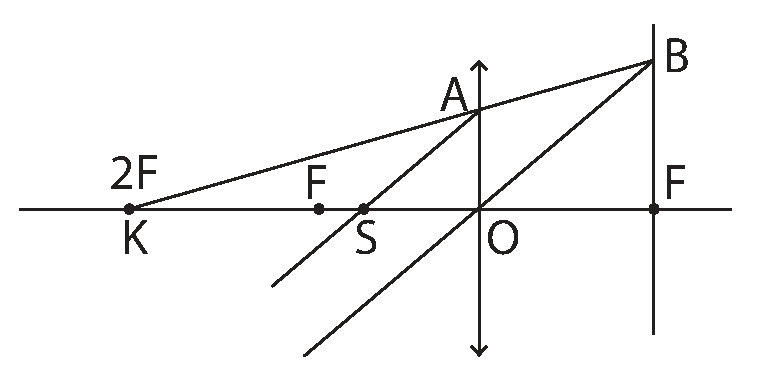
\includegraphics[width=0.7\linewidth]{2018-v2g-02-valgusallikaslah}
 \end{center}
 \vspace{-10pt}

Sarnastest kolmnurkadest $\triangle KAO$ ja $\triangle KBF$ saame, et
\[ \frac{AO}{BF} = \frac{KO}{KF} = \frac{2f}{3f} = \frac{2}{3}. \]
Teisest sarnaste kolmnurkade paarist $\triangle SAO$ ja $\triangle OBF$ saame, et
\[ \frac{AO}{BF} = \frac{OS}{FO} = \frac{b}{f}, \]
kus b on teise valgusallika kaugus läätsest. Ühendades kaks seost, saame
\[ \frac{KO}{KF}=\frac{OS}{FO} \quad\Rightarrow\quad \frac{2}{3} = \frac{b}{f} \quad\Rightarrow\quad b = \frac{2f}{3} = \SI{6}{cm}. \]
Teine valgusallikas peab asuma läätsest \SI{6}{cm} kaugusel ning kahe valgusallika kaugus teineteisest on \SI{6}{cm} + \SI{18}{cm} = \SI{24}{cm}.

\vspace{\baselineskip}
\emph{Teine lahendus}\\
Sarnaste kolmnurkade asemel saame kasutada läätse valemit. Teades, et valgusallikas asub läätsest $a = \SI{18}{cm}$ kaugusel ning läätse fookuskaugus on $f=\SI{9}{cm}$, saame leida kujutise kauguse $k$ läätsest:
\[ \frac{1}{a} + \frac{1}{k} = \frac{1}{f} \quad\Rightarrow\quad k = \SI{18}{cm}. \]
Teise valgusallika kujutis peab olema samuti samas punktis, kus esimese valgusallika oma, seega peab teise valgusallikaga tekitatud kujutis olema näiline ning valgusallikas peab asuma kujutisega samal pool läätse. Kasutades läätse valemit, leiame teise valgusallika asukoha
\[ \frac{1}{a} - \frac{1}{k} = \frac{1}{f} \quad\Rightarrow\quad a = \SI{6}{cm}. \]
Teine valgusallikas peab asuma läätsest \SI{6}{cm} kaugusel ning kahe valgusallika kaugus teineteisest on \SI{6}{cm} + \SI{18}{cm} = \SI{24}{cm}.

\probeng{Two light sources}
Two point light sources are positioned on different points of a convex lens’ optical axis. The images of these light sources formed by the lens coincide. It is known that one light source is at a distance $a=\SI{18}{cm}$ from the center of the lens. How far is the other light source distanced from this light source? The focal length of the lens is $f=\SI{9}{cm}$.

\hinteng
For the two light sources to give the same image one of them has to be virtual and the other real.

\solueng
\emph{First solution}\\
If the light source located on the optical axis is at the distance of 18 cm from the lens which is equal to double the focal length then the image of the light source is located on the other side of the lens also at double the focal length from the lens, meaning at the distance 18 cm. For the images of the two light sources to coincide the other image has to be virtual. Let us construct the location of the light source if the location of the image is known.
\begin{center}
    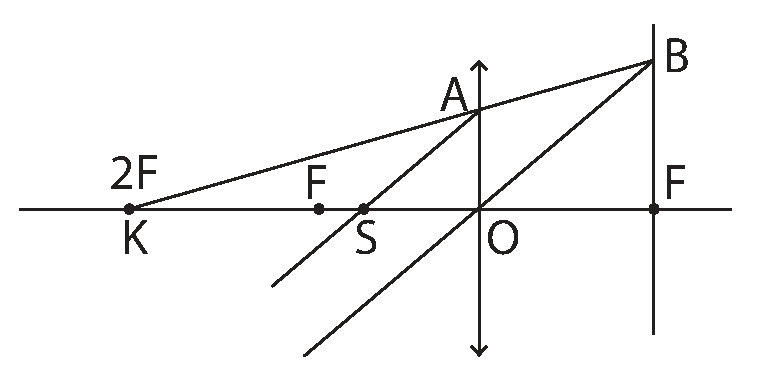
\includegraphics[width=0.7\linewidth]{2018-v2g-02-valgusallikaslah}
  \end{center}
From the similar triangles $\triangle KAO$ and $\triangle KBF$ we get that
\[ \frac{AO}{BF} = \frac{KO}{KF} = \frac{2f}{3f} = \frac{2}{3}. \] 
From the other pair of similar triangles $\triangle SAO$ and $\triangle OBF$ we get that
\[  \frac{AO}{BF} = \frac{OS}{FO} = \frac{b}{f},  \] 
where b is the distance of the second light source from the lens. Connecting the two relations we get
\[ \frac{KO}{KF}=\frac{OS}{FO} \quad\Rightarrow\quad \frac{2}{3} = \frac{b}{f} \quad\Rightarrow\quad b = \frac{2f}{3} = \SI{6}{cm}. \] 
The second light source has to be located from the lens at a distance 6cm and the distance between the two light sources is $\SI{6}{cm} + \SI{18}{cm} = \SI{24}{cm}$. \\

\emph{Second solution}\\
Instead of similar triangles we can use the thin lens formula. Knowing that the light source is at the distance $a = \SI{18}{cm}$ from the lens and the focal length of the lens is $f=\SI{9}{cm}$ we can find the distance $k$ of the image from the lens:
\[ \frac{1}{a} + \frac{1}{k} = \frac{1}{f} \quad\Rightarrow\quad k = \SI{18}{cm}. \] 
Since the images of the two light sources have to coincide then the image made by the second light source has to be virtual and the light source has to be located at the same side of the lens as the image. Using the thin lens formula we find the location of the second light source 
\[ \frac{1}{a} - \frac{1}{k} = \frac{1}{f} \quad\Rightarrow\quad a = \SI{6}{cm}. \] 
The second light source has to be at the distance 6 cm from the lens and the distance between the two light sources is $\SI{6}{cm} + \SI{18}{cm} = \SI{24}{cm}$.
\probend